\setchapterpreamble[u]{\margintoc}
\glsresetall % reset glossary
\todo{tables always small}

\chapter{Design of real-size aeronautical wing structures}
Introduction
Ultralight trusses are a good design candidate for the design of innovative aerostructures thanks to their superior aeroelastic properties and stiffness-to-weight ratio \cite{cramer_elastic_2019}. These structures represent a natural application case for the discussed optimization formulations. \cite{opgenoord_aeroelastic_2018, opgenoord_design_2019} proposed a two-step sequential optimization algorithm to reduce the weight of a truss wing. Firstly, a ground structure with different nodal densities based on the stress field of the structure is generated and secondly, the cross-sectional areas are found using a sizing optimization algorithm that takes into account stress, local buckling, and aeroelastic constraints. \cite{shahabsafa_novel_2018} decided, instead, to tackle all the difficulties of the problem using a set of discrete cross-sectional areas and a sizing \gls{milo} algorithm. The algorithm is validated on a 315-bars wingbox ground structure, based on the \gls{crm}. In these studies, the adoption of a sizing optimization algorithm simplifies the numerical complexities associated with the problem. However, by solely focusing on modifying the component sizes, the opportunity to optimize the overall truss topology is missed, limiting the potential for further weight savings.
\section{3D CRM wingbox with multiple load cases}

In this section, the proposed strategy is used to optimize a real-size wingbox, to validate its ability to work on large, three-dimensional structures with more candidate members compared to the precedent test cases. The structure is based on the jig (undeformed) shape of the wingbox of the NASA \gls{crm} \cite{brooks_benchmark_2018}. The structure is submitted to three different load cases: +2.5 g maneuver (LC\_1), -1 g maneuver (LC\_2), and cruise with gust +1.3 g (LC\_3). The nodes of the bounding volume and the loads used are provided by \cite{fakhimi_discrete_2021}, where a detailed discussion on how they are evaluated can be found. The ground structure of the test case is presented in \figref{fig:crm315_x0}.

The material used for the optimization is an aluminum alloy with Young's modulus of \qty{69}{\GPa}, density of \qty{2.7}{\gram/\cm^3}, and yield stress equal to $\pm$\qty{270}{\MPa}. To ensure a conservative design, we incorporated safety factors (\textit{sf}) associated with each load case. These safety factors were integrated into the formulation by reducing the maximum stress and buckling allowables by factors of 1.5, 1.5, and 2.67 for the three considered load cases, respectively. No bounds constraints are imposed on the nodal displacements of the structure and the cross-sections are assumed circular with the $s$ parameter of \eqref{eq:s} $s = \pi E/4$. The optimization is carried only on the wingbox, the internal structure of the wing, and there is no influence of the skin on the optimization.

\subsection{Advanced thresholding}
As the \gls{crm} is a large and thin structure that presents a noticeable difference in load magnitude between the tip and the root of the wingbox, the quantities of interest of the optimization span different orders of magnitude (from \unit{m^2} to \unit{mm^2}, and from \unit{MN} to \unit{N}). For that reason, the choice of the cross-sectional area threshold value $\chi$ of Equation \eqref{eq:thr} used to simplify the initial \gls{nlp} ground structure is crucial. Taking a high value (such as $\chi = 10^{-4}$, restraining the solution from \unit{m^2} to \unit{cm^2}) would mean possibly canceling out bars fundamental for the nodal force equilibrium in the less loaded part of the wing (wing tip and the central part of the wing's sections near the root). By contrast, a low value (such as $\chi=10^{-9}$) would permit the correct simulation of the mechanical response of the structure, but it would lead to a very high number of candidate bars and, thus, longer optimizations and convergence difficulty for the \gls{nlp} phase. For that reason, $\chi$ is set to an average value ($\chi=10^{-6}$), eliminating all the bars under the value $a_{\text{thr}}=\chi \; \max(\vect{a})$, but an additional check is performed before proceeding to the thresholding. The bars under the threshold $a_{\text{thr}}$ are sorted in ascending order of cross-sectional area and, starting from the smallest one, we iteratively check via a \gls{fea} that the difference between the force and displacement fields before and after the bar removal is below than a certain bound. In the present study we used the following: $\norm{\Delta q}_{\infty}<\qty{10}{N}$ and $\norm{\Delta U}_{\infty}<\qty{1}{cm}$.

\subsection{Numerical application}

\begin{table}
    \centering
    \begin{tabular}{ccc}
    \toprule
    \textbf{Quantity} & \textbf{CRM-315} & \textbf{CRM-2370} \\ \midrule
    N$_{\text{el}}$          & 315               & 2370               \\
    N$_{\text{opt}}$           & 257                  &  1127              \\
    V [\unit{\meter^3}]             &  7.90                 &  7.44             \\
    V [\unit{\%}]             &   \qty{1.309}{\%}                & \qty{1.232}{\%}               \\
    Mass [\unit{\tonne}]               &   21.342                & 20.092     \\
    a$_{\text{max}}$ [\unit{\meter^2}]           &  0.198                 & 0.208              \\
    C$_\text{LC\_1}$ [\unit{\mega \joule}]                &  3.23                 &  3.17              \\
    C$_\text{LC\_2}$ [\unit{\mega \joule}]                &   1.28                &  1.27              \\
    C$_\text{LC\_3}$ [\unit{\mega \joule}]                &   0.76                &  0.74              \\
    t [\unit{\second}]                & 147                  & 3189   \\ \bottomrule            
    \end{tabular}
    \caption{Numerical results of the optimization of the CRM with two different ground structures.}
    \label{tab:wing-res}
    \end{table}
    
    \begin{figure*}
        \centering
        \subcaptionbox{\label{fig:crm315_x0}}{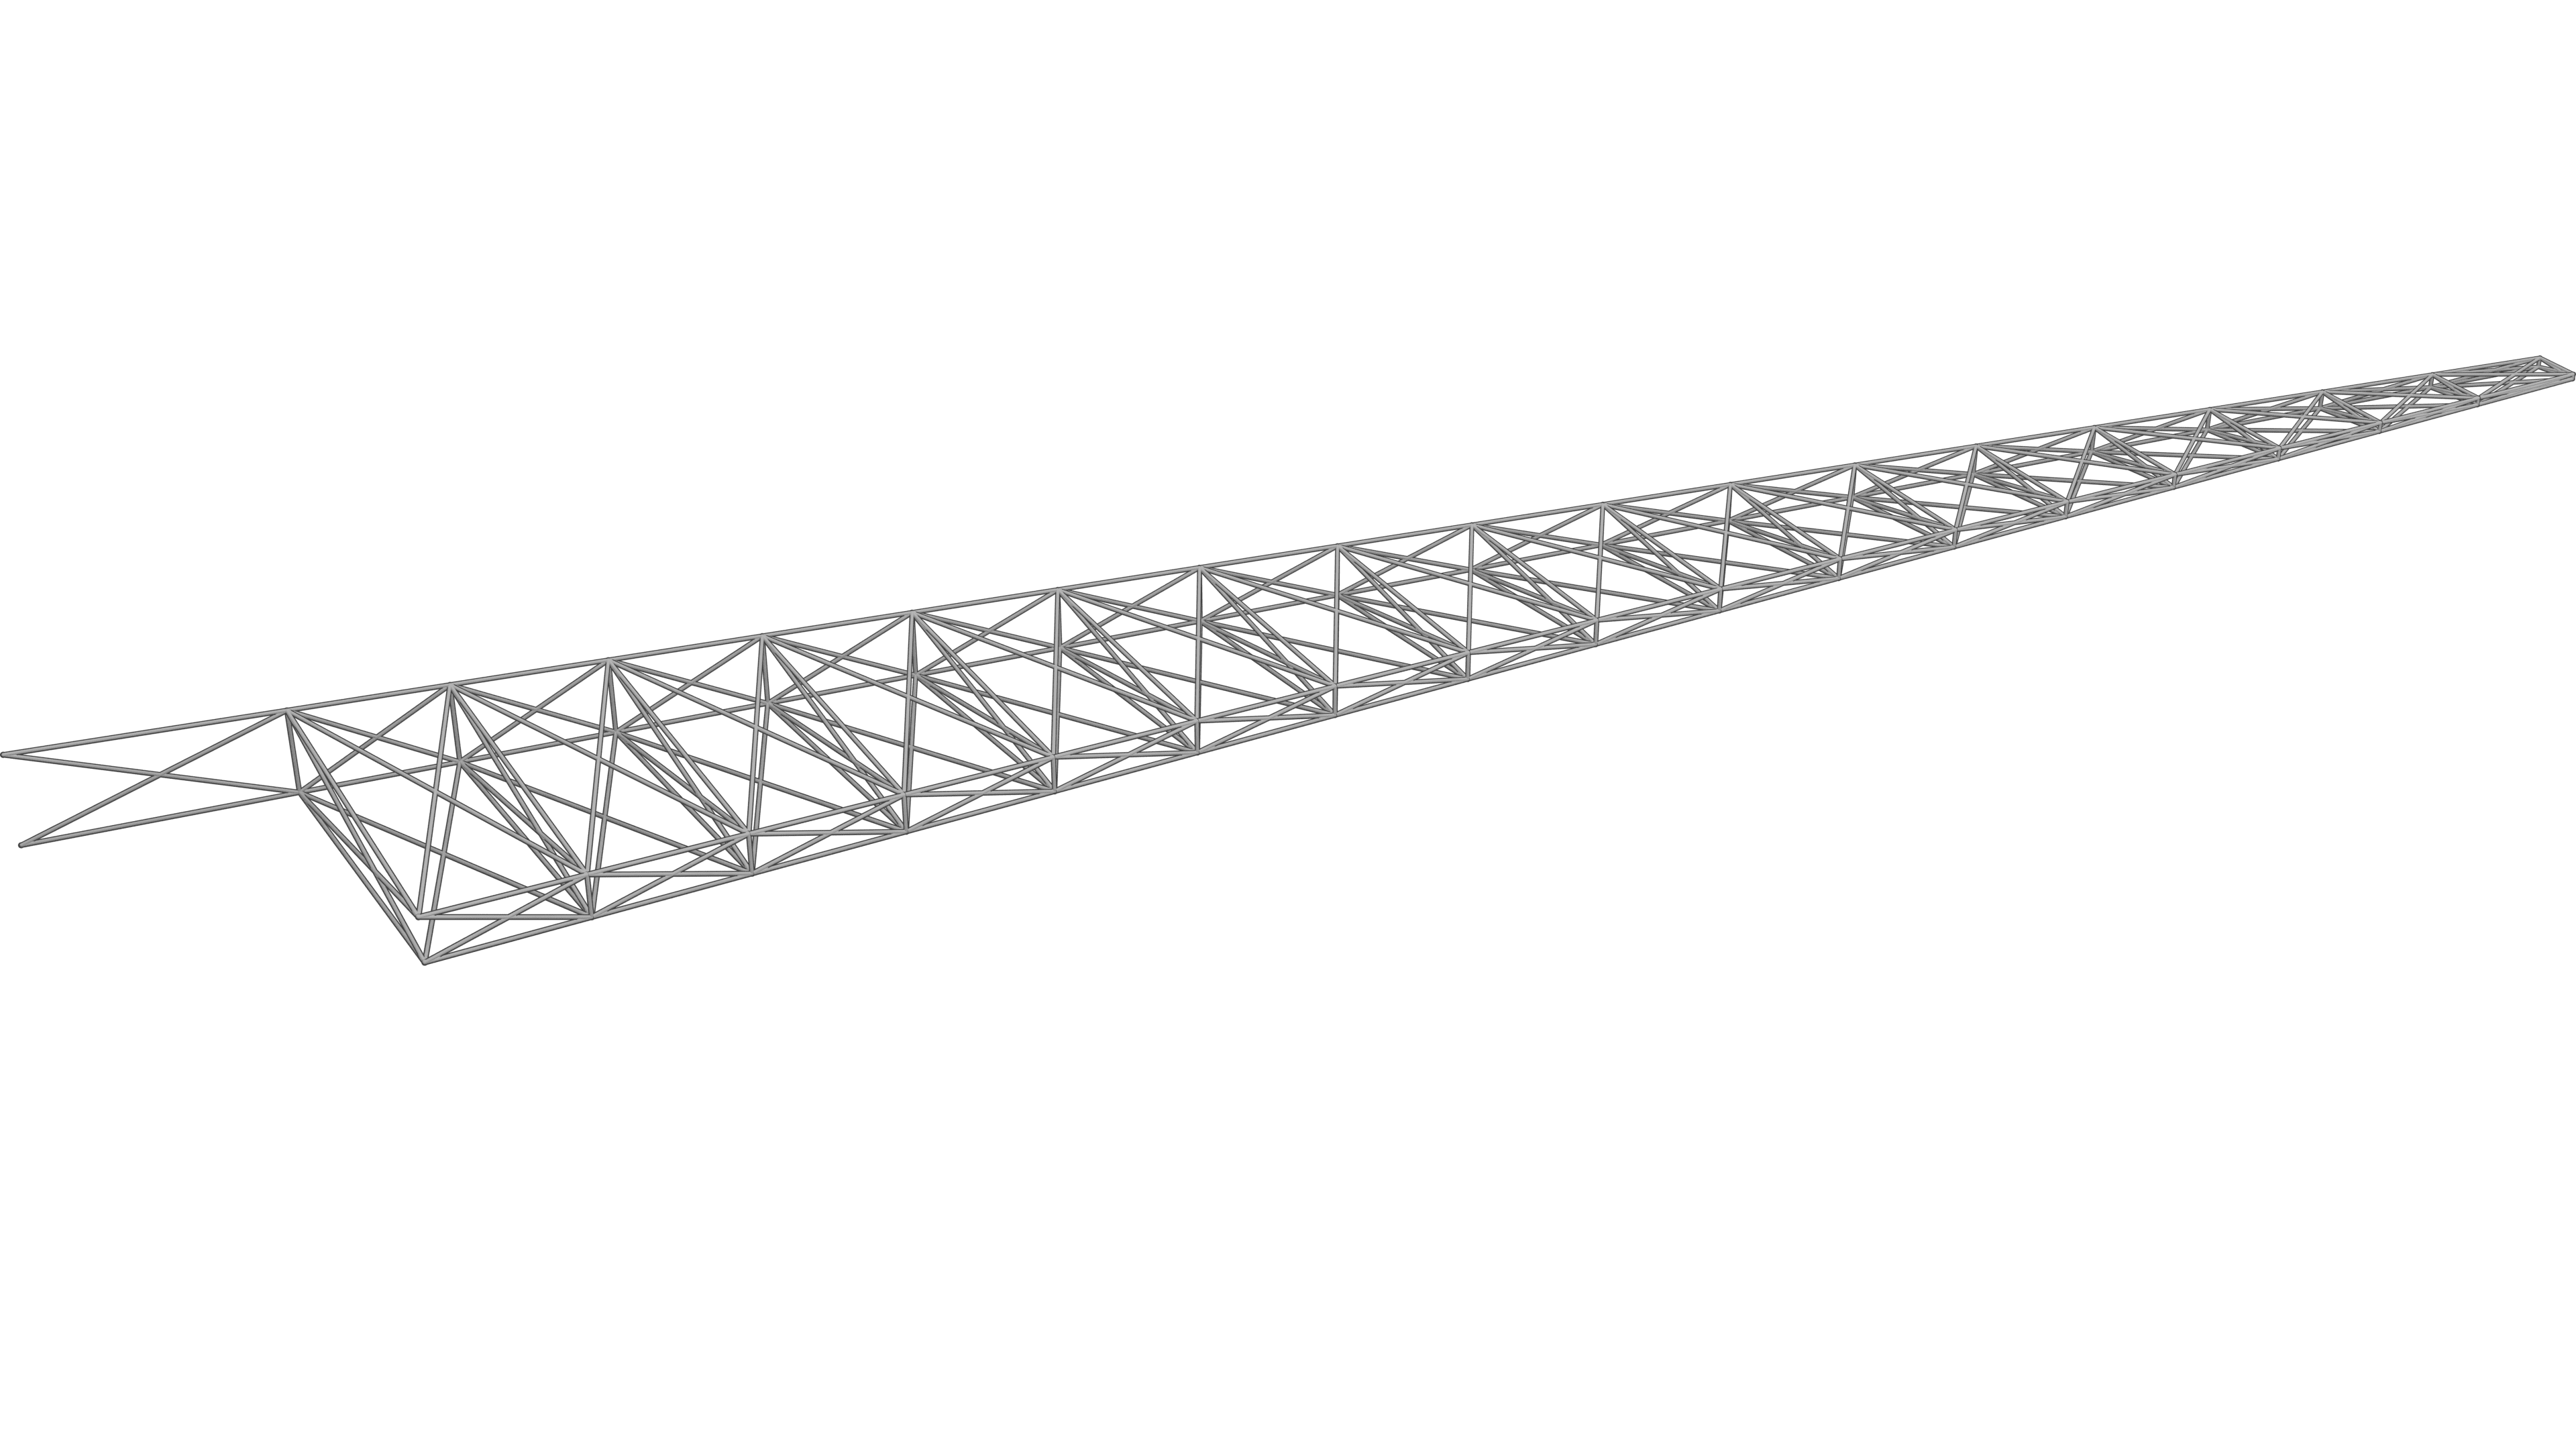
\includegraphics[width=0.45\textwidth]{14a_00_Topology_x0_iso.png}}
        \bigskip
        \subcaptionbox{\label{fig:crm2317_x0}}{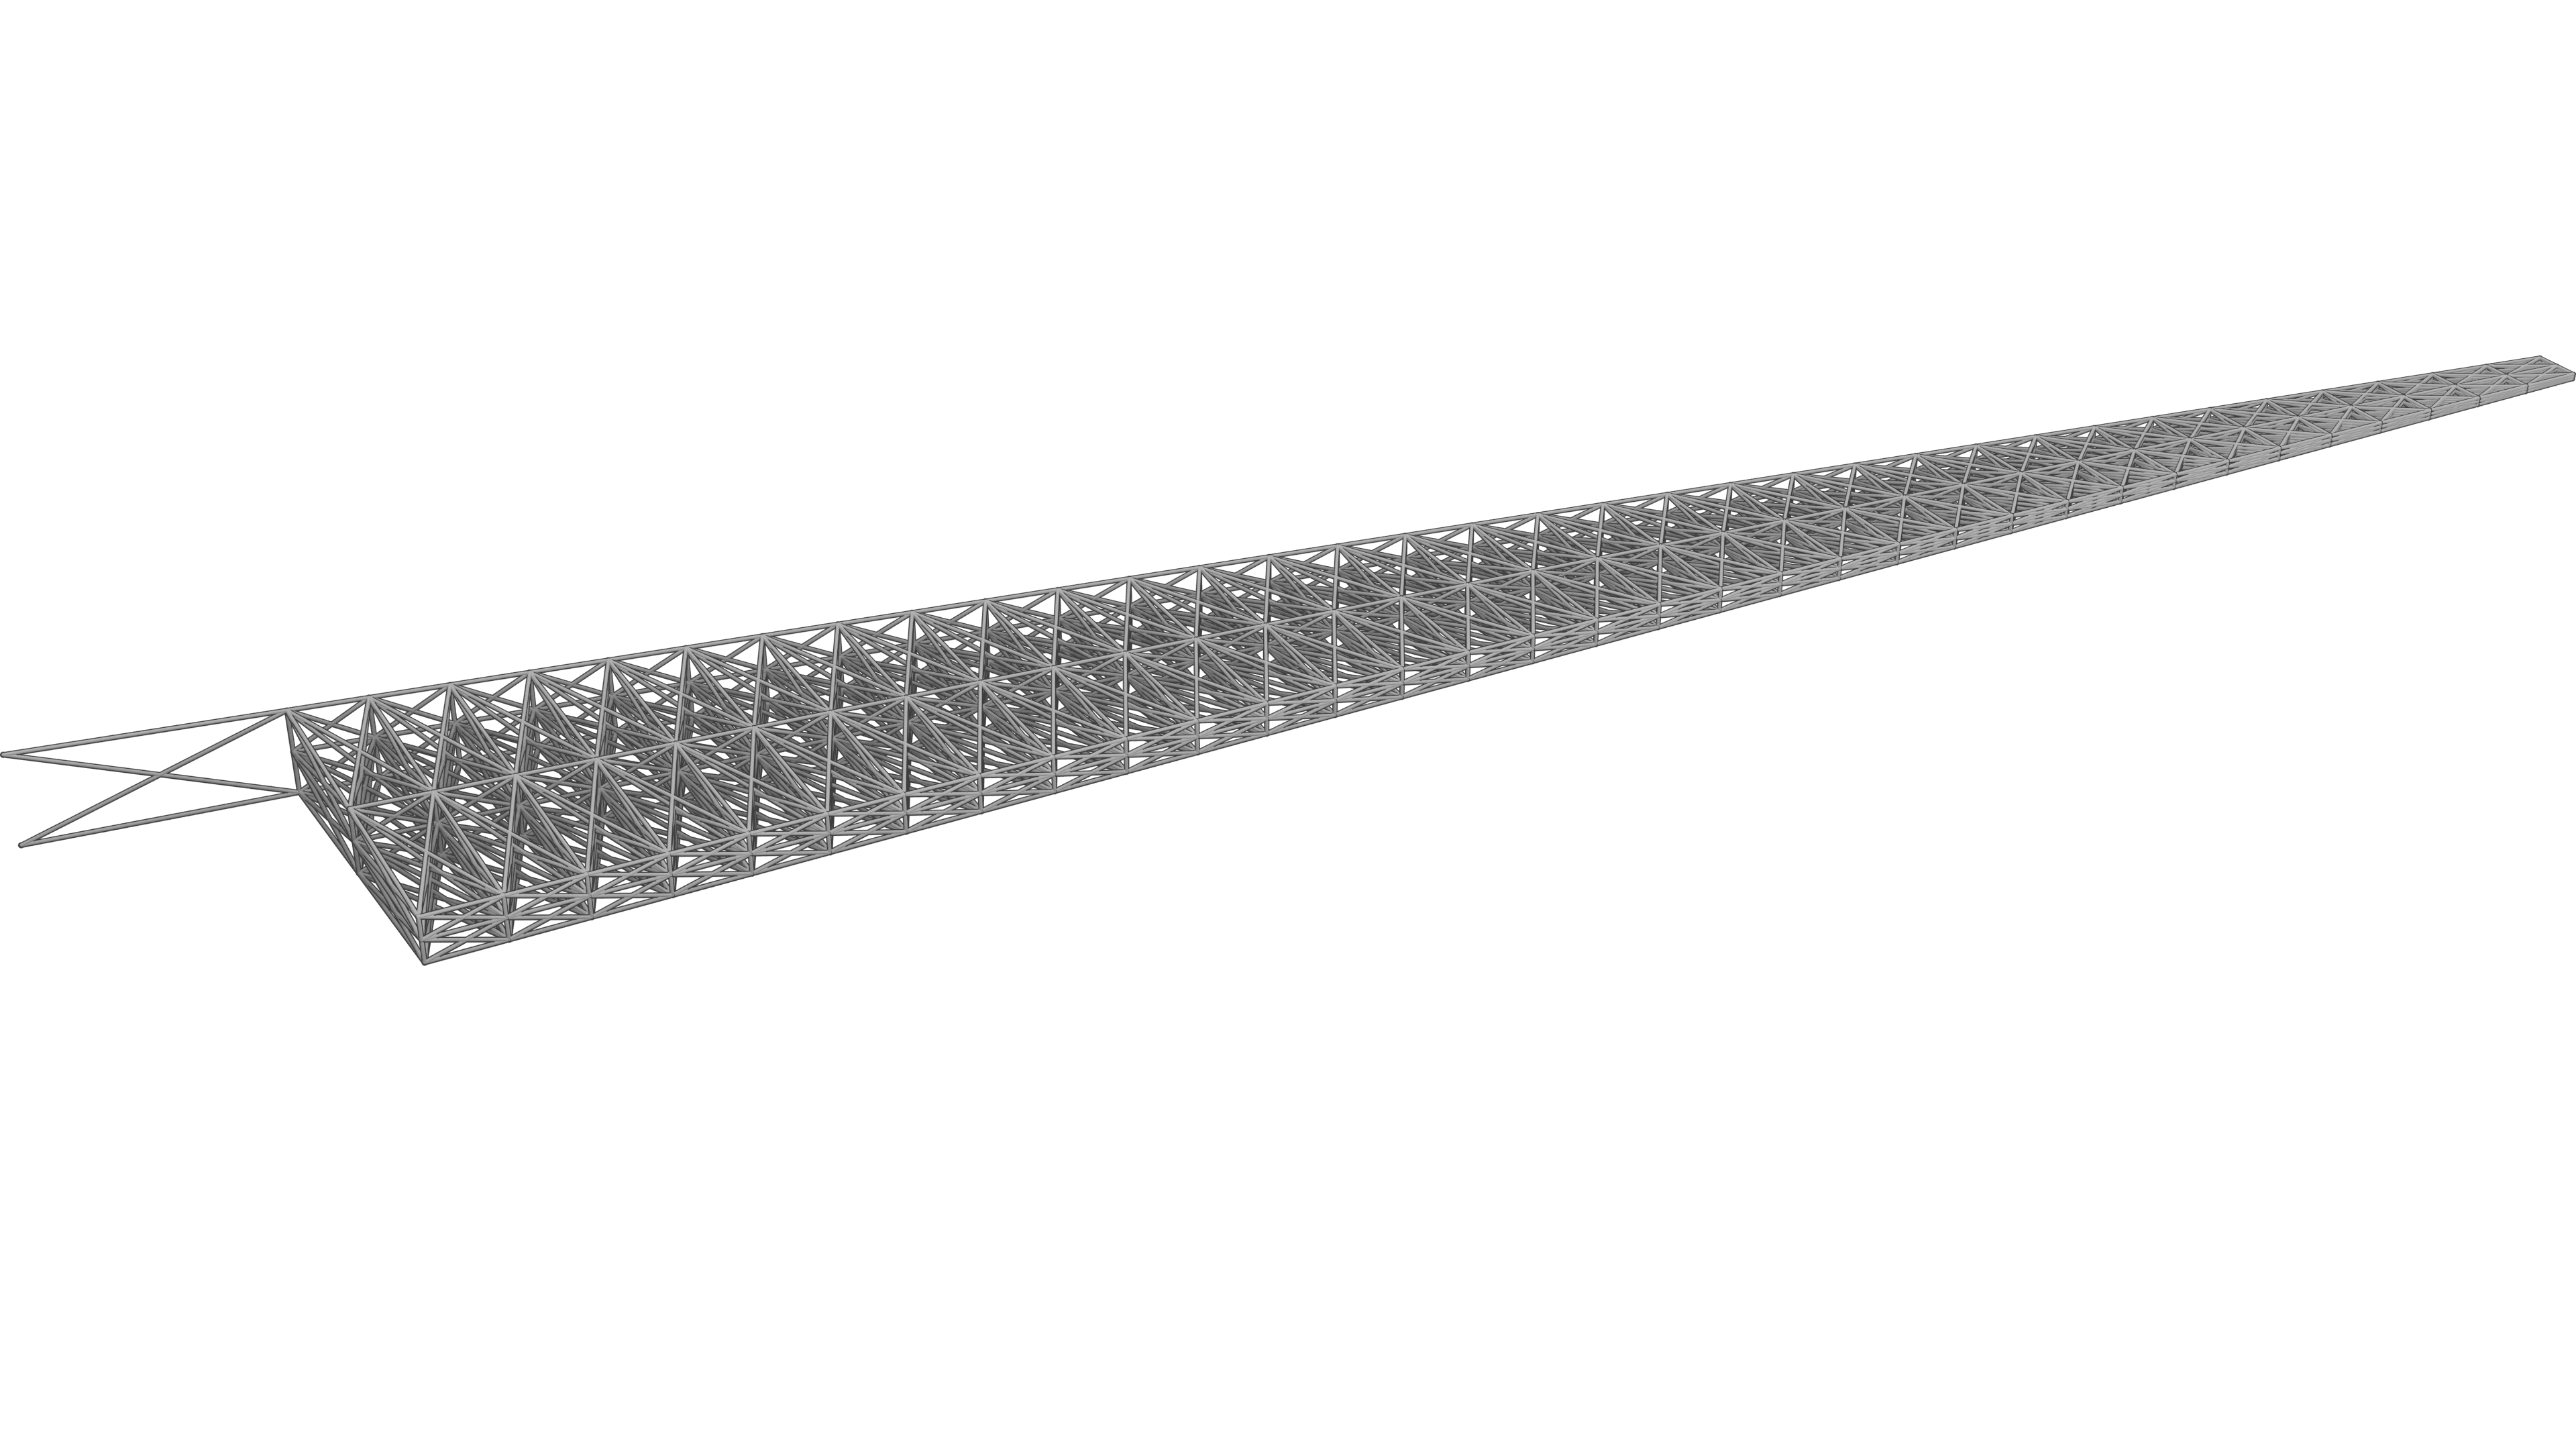
\includegraphics[width=0.45\textwidth]{14b_00_Topology_x0_iso 2370.png}}
        \caption{(a) Ground structure of the CRM-315 test case; (b) Ground structure of the CRM-2370 test case. The cross-sectional areas shown in the two sub-figures represent the starting point of the optimizations.}
        \label{fig:crm}
    \end{figure*}
    
    \begin{figure}
        \centering
        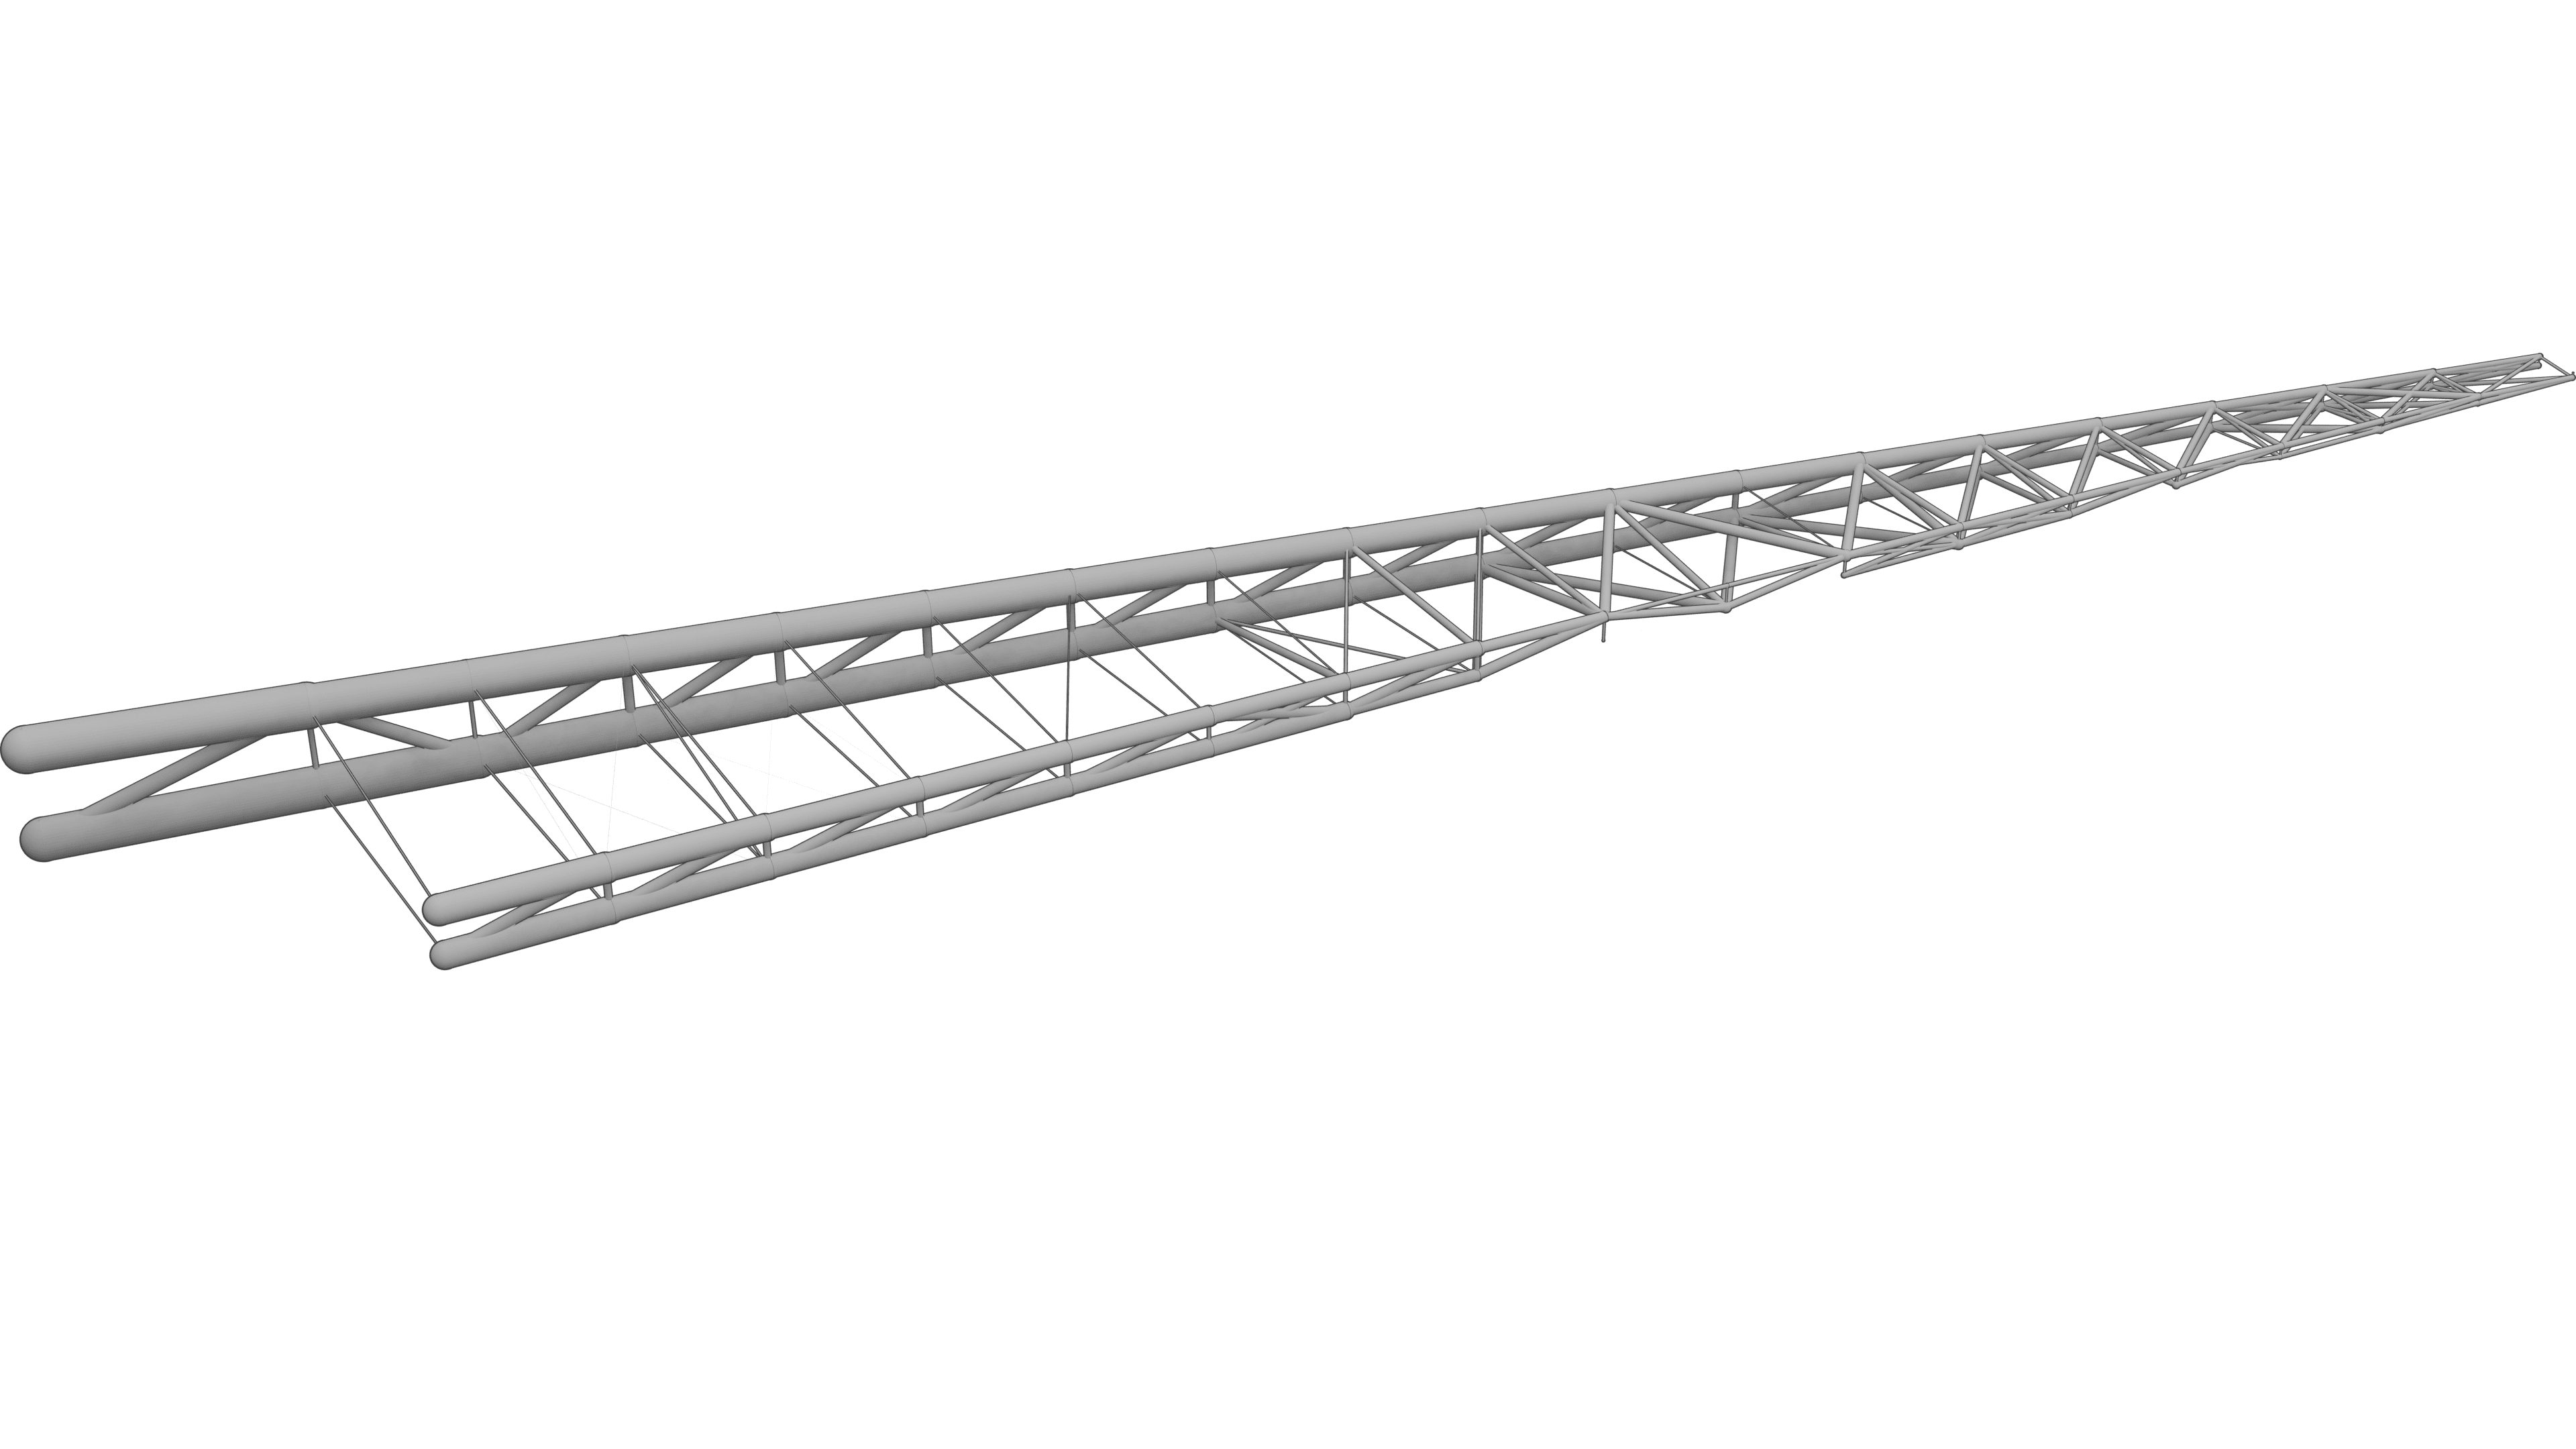
\includegraphics[width=0.5\textwidth]{15_04_Topology_NLP_iso.png}
         \caption{Optimized topology of the CRM-315 with 257 active bars.}
        \label{fig:crm315}
    \end{figure}
    
    Two different discretizations are considered for the optimization. The proposed algorithm is firstly tested on the same ground structure provided by \cite{fakhimi_discrete_2021}, composed of $N_{\text{el}}=315$ candidate members (CRM-315). The second discretization is obtained by refining the 315-bar ground structure, evaluating the midpoints of every member, and connecting them with first-order connectivity. We obtain $N_{\text{el}}=2370$ candidate members (CRM-2370). The loads and the boundary conditions are applied on the same nodes of the ground structure for the two studied ground structures. The cross-sectional areas of the starting point of the CRM-315 and the CRM-2370 are set to \qty{0.0001}{m^2} and they are shown in \figref{fig:crm}. Only one single start point is used for these two examples as the proposed two-step strategy with reinitialization already proved in the previous sections to reduce the starting point influence on the optimization result. The resolution algorithm used is 2S-5R. The numerical results of the optimization for the two different discretizations are reported in \tabref{tab:wing-res}. 
    
    The optimized CRM-315 structure shows a mass of \qty{21.342}{\tonne}, a \qty{27.01}{\%} reduction compared to the solution with discrete cross-section areas found by \cite{fakhimi_discrete_2021}  (\qty{29.238}{\tonne}). Other than the substantial difference in the modelization of the cross-section areas, the mass reduction could be explained by the fact that the proposed algorithm has a zero lower bound on cross-sectional areas, thus permitting the topology of the structure to change: the 2S-5R solution shows 257 active bars out of 315 at convergence (see \figref{fig:crm315}). In contrast, the \gls{milo} problem solved by \cite{fakhimi_discrete_2021} is employed as a sizing optimization algorithm with fixed topology (and thus 315 active members in the optimized design). A more detailed comparison could not be performed as the authors did not share the values of the cross-sectional areas of their solution. 
    
    The volume fraction of the solution is \qty{1.313}{\percent} and the minimum slenderness ratio $\lambda$ (ratio between the length and the radius of gyration of the bar) of a bar is 14.96, which is compatible with the truss modelization used to discretize the wingbox volume. The execution time of the optimization is \qty{19}{s} for the \gls{slp} step and \qty{128}{s} for the \gls{nlp} step, for a total of \qty{147}{s} on a regular notebook, compared to the over four days of optimization of \cite{fakhimi_discrete_2021} on a desktop workstation. The iteration history curves of the optimization are plot in \figref{fig:c2}.

\paragraph{Maximum displacements constraints}

\paragraph{Multiple materials}
\todo{complete with Ashby charts on cost and co2 evaluation}

\paragraph{Enriching the mesh}
\begin{figure*}
    \centering
    \includegraphics[width=\textwidth]{16_wing_opt.pdf}
     \caption{Maximum stress constraint value (left) and buckling constraint value (right) plotted on the deformed shape of the optimized design (undeformed shape in light grey) of CRM-2370 for the three load cases: +2.5 g maneuver (a), -1 g maneuver (b), and cruise with gust (+1.3 g) (c). The maximum $z$ tip deflection is \qty{4.167}{m}, \qty{-2.953}{m}, and \qty{1.948}{m}, respectively.}
    \label{fig:wing_opt}
\end{figure*}
The mass of the optimized CRM-2370 structure is \qty{20.092}{\tonne}, a \qty{1.318}{\tonne} reduction compared to the CRM-315 (\qty{-6.2}{\%}). Additionally, if we compare the compliance of the three load cases (see \tabref{tab:wing-res}), we notice how the solution of CRM-2370 is not only lighter but also stiffer, suggesting in general a more efficient structure topology. The maximum z tip deflection of the wingbox is \qty{4.167}{m}, \qty{-2.953}{m}, \qty{1.948}{m} for the three considered load cases, respectively. There are 1127 active bars in the optimized design, and the whole optimization took \qty{3189}{s} (\qty{1911}{s} for the \gls{slp} step, \qty{1278}{s} for the \gls{nlp} step). The iteration history curves of the optimization are plot in \figref{fig:c3}. In \figref{fig:wing_opt} the normalized maximum stress and buckling constraints are plotted on the deformed shape of the three load cases. We notice how in general the topology of the two external "spars" is shaped after the +2.5 g load case, while the interior of the wingbox is made by a thinner truss constrained by buckling. 

\paragraph{Active mechanical constraints}
To better understand which mechanical phenomena is the most constraining for the bars of the solution, we present in \figref{fig:fail-crm} a graph where the normalized stress criterion $\vect{c_s}=\max{\left(-\vect{q} \; \textit{\textbf{sf}}/\sigma_c \vect{a},\vect{q} \; \textit{\textbf{sf}}/\sigma_t \vect{a}\right)}$ and the normalized buckling criterion $\vect{c_b}=\vect{q}\; \textit{\textbf{sf}}/\vect{q}_{\text{crit}}$ are plotted against each other. Every point in the scatter plot represents the members of the solution of the \gls{slp} and the \gls{nlp} steps that show at least a charge of 1N (931 out of 1127 members). This threshold is applied as at the end of the NLP step some members present a very small section, creating numerical problems when evaluating the stress and buckling criteria. All the \gls{slp} members activate either the maximum stress or buckling limit, while 68 out of 931 \gls{nlp} members are located in the center of the graph ($c_s<0.95$ and $c_b<0.95$). We speculate that this behavior is due to the inclusion of the kinematic compatibility constraint in the \gls{nlp} algorithm: the cross-sectional area of these bars is chosen to comply with the global displacements. In \tabref{tab:constrNLP}, a summary of the active mechanical failure constraints (buckling, tensile stress, and compressive stress) present in the NLP solution. The table showcases the number of active constraints categorized by constraint type and load case. The optimized design encompasses a total of 930 active mechanical failure constraints for 863 bars (931 minus the 68 bars constrained by kinematic compatibility). This suggests that certain members are concurrently subject to multiple failure constraints across different load cases. An additional observation is that the design of the solution is primarily influenced by local buckling and compressive failures, especially under the +2.5 g load case (LC\_1).

\begin{figure}
    \centering
    \includegraphics[width=0.5\textwidth]{17_failure_max.pdf}
     \caption{Normalized buckling and maximum stress constraint values for the optimized CRM-2370 structure after the SLP and the NLP optimization steps.}
    \label{fig:fail-crm}
\end{figure}

\begin{table}
\centering
\begin{tabular}{lS[table-format=3.0]S[table-format=3.0]S[table-format=3.0]S[table-format=3.0]S[table-format=3.0]}
\toprule
                     & \textbf{LC\_1} & \textbf{LC\_2} & \textbf{LC\_3} & \textbf{Tot.} \\ \midrule
\textbf{Buckling}    & 281           & 145           & 143           & 569           \\
\textbf{Tension}     & 56            & 3             & 4             & 63            \\
\textbf{Compression} & 286           & 6             & 6             & 298           \\
\midrule
\textbf{Tot.}        & 623           & 154           & 153           & 930          \\
\bottomrule
\end{tabular}
\caption{Number of active mechanical failure constraints for the CRM-2370 optimized design per type of constraint (rows) and per load case (columns).}
\label{tab:constrNLP}
\end{table}

\section{NACA profile extruded}

\subsection{Numerical implementation}

\subsection{Meshing irregular volumes}

\subsection{Definition of the repetitive zones}

\subsection{Numerical application}

\section{Conclusion}